% ============================================================================
% PHASE 1 PROGRESS REPORT — Beamer Presentation
% Design matches state_of_the_art_final.tex
% ============================================================================
\documentclass[aspectratio=169, dvipsnames]{beamer}
\usetheme{SimplePlus}

% Packages (same as state_of_the_art_final.tex)
\usepackage[utf8]{inputenc}
\usepackage{subcaption}
\usepackage{hyperref}
\usepackage{amsmath}
\usepackage{xcolor}
\usepackage{graphicx}
\usepackage{booktabs}
\usepackage{tikz}
\usepackage{fontawesome5}

\usetikzlibrary{arrows.meta, positioning, calc, shapes.geometric}

% ============================================================================
% TITLE PAGE INFO
% ============================================================================
\title[Phase 1 Progress]{Phase~1 Progress Report}
\subtitle{Objective~1 — Robust Pipeline for Longitudinal Cancer Imaging}
\author[M. BOUFAFA]{
    \textbf{Mohamed BOUFAFA}\\
    \vspace{0.3em}
    {\small Mitacs Globalink Research Internship}
}
\institute[TÉLUQ]{
    \textbf{TÉLUQ University}, Montreal\\
    \vspace{0.3em}
    \footnotesize
    Supervisor: Dr.\ Belkacem Chikhaoui (TÉLUQ)\\
    Co-supervisor: Dr.\ Belkacem Khaldi (Algeria)
}
\date{July 2025}

\begin{document}

% ============================================================================
% TITLE SLIDE
% ============================================================================
\begin{frame}[plain]
    \maketitle
\end{frame}

% ============================================================================
% SLIDE 1: Roadmap
% ============================================================================
\begin{frame}{Roadmap}
    \begin{columns}
        \begin{column}{0.48\textwidth}
            \begin{block}{\faIcon{route} This Presentation}
                \begin{enumerate}
                    \item Where we are in Phase~1
                    \item What has been completed
                    \item Key technical decisions
                    \item What remains
                    \item Timeline to Phase~2
                \end{enumerate}
            \end{block}
        \end{column}

        \begin{column}{0.48\textwidth}
            \begin{exampleblock}{\faIcon{bullseye} Phase 1 Goal}
                Build a reproducible pipeline that takes \textbf{raw multi-scanner brain MRIs} and outputs \textbf{clean, segmented, temporally aligned} longitudinal sequences ready for deep learning.
            \end{exampleblock}

            \vspace{0.3em}

            \begin{alertblock}{\small Current Status}
                \textbf{4 of 6 steps complete.}\\
                Segmentation model configured \& validated.\\
                Registration notebook to be created.
            \end{alertblock}
        \end{column}
    \end{columns}
\end{frame}

% ============================================================================
% SLIDE 2: Pipeline Overview with Progress
% ============================================================================
\begin{frame}{Phase~1 Pipeline — Progress at a Glance}
    \begin{center}
        \begin{tikzpicture}[
            box/.style={rectangle, draw=#1, fill=#1!10, thick, minimum height=0.85cm, minimum width=2.3cm, align=center, rounded corners, font=\scriptsize},
            done/.style={rectangle, draw=ForestGreen, fill=ForestGreen!15, thick, minimum height=0.85cm, minimum width=2.3cm, align=center, rounded corners, font=\scriptsize},
            todo/.style={rectangle, draw=red!60, fill=red!8, thick, minimum height=0.85cm, minimum width=2.3cm, align=center, rounded corners, font=\scriptsize, dashed},
            arr/.style={->, thick, >=stealth, color=gray!70},
            chk/.style={font=\scriptsize, color=ForestGreen!80!black},
            cross/.style={font=\scriptsize, color=red!70!black}
        ]

        % Row 1: Steps
        \node[done] (audit) at (0,0) {\textbf{Data Audit}\\{\tiny 1,430 patients}};
        \node[done] (prep) at (3.2,0) {\textbf{Preprocess}\\{\tiny Register + Resample}};
        \node[done] (eda) at (6.4,0) {\textbf{EDA / QC}\\{\tiny Quality Check}};

        \draw[arr] (audit) -- (prep);
        \draw[arr] (prep) -- (eda);

        % Row 2: Steps
        \node[done] (cnn) at (0,-2) {\textbf{CNN Baseline}\\{\tiny 3D CNN + Grad-CAM}};
        \node[done] (seg) at (3.2,-2) {\textbf{Segmentation}\\{\tiny nnU-Net BraTS2021}};
        \node[todo] (reg) at (6.4,-2) {\textbf{Registration}\\{\tiny itk-elastix}};

        \draw[arr] (eda) -- ++(0.8,0) |- (cnn);
        \draw[arr] (cnn) -- (seg);
        \draw[arr] (seg) -- (reg);

        % Check marks
        \node[chk] at (0,0.7) {\faIcon{check-circle} NB\,01};
        \node[chk] at (3.2,0.7) {\faIcon{check-circle} NB\,02};
        \node[chk] at (6.4,0.7) {\faIcon{check-circle} NB\,03};
        \node[chk] at (0,-1.3) {\faIcon{check-circle} NB\,04};
        \node[chk] at (3.2,-1.3) {\faIcon{check-circle} NB\,05};
        \node[cross] at (6.4,-1.3) {\faIcon{times-circle} NB\,06};

        % Output arrow
        \node[box=RoyalBlue] (out) at (9.8,-2) {\textbf{Phase 2}\\{\tiny Swin UNETR}};
        \draw[arr] (reg) -- (out);

        \end{tikzpicture}
    \end{center}

    \vspace{0.5em}

    \begin{columns}
        \begin{column}{0.32\textwidth}
            \centering
            \scriptsize
            \textcolor{ForestGreen}{\faIcon{check}} \textbf{5 notebooks} complete\\
            Code written \& validated
        \end{column}
        \begin{column}{0.32\textwidth}
            \centering
            \scriptsize
            \textcolor{ForestGreen}{\faIcon{check}} \textbf{All outputs} saved\\
            CSV, JSON, figures, reports
        \end{column}
        \begin{column}{0.32\textwidth}
            \centering
            \scriptsize
            \textcolor{red}{\faIcon{clock}} \textbf{1 notebook} remaining\\
            Longitudinal registration
        \end{column}
    \end{columns}
\end{frame}

% ============================================================================
% SLIDE 3: Dataset Summary
% ============================================================================
\begin{frame}{Dataset: Yale Brain Metastases — Key Numbers}
    \begin{columns}
        \begin{column}{0.50\textwidth}
            \begin{block}{Inventory Results (Notebook~01)}
                \small
                \begin{tabular}{ll}
                    \toprule
                    \textbf{Metric} & \textbf{Value} \\
                    \midrule
                    Patients & 1,430 \\
                    Total visits & 11,877 \\
                    Total NIfTI files & 33,811 \\
                    Disk size & $\sim$43\,GB \\
                    Modalities & FLAIR, T1, T1c, T2 \\
                    \midrule
                    Complete visits (4/4 mod.) & 4,405 (37.1\%) \\
                    Patients with $\geq$3 visits & 1,126 \\
                    Patients with $\geq$10 visits & 271 \\
                    \midrule
                    Median follow-up & 345 days \\
                    Max follow-up & 5,061 days \\
                    \bottomrule
                \end{tabular}
            \end{block}
        \end{column}

        \begin{column}{0.46\textwidth}
            \begin{alertblock}{Key Challenge}
                \small
                Only \textbf{37.1\%} of visits have all 4 modalities.\\[0.3em]
                nnU-Net requires all 4 $\Rightarrow$ \textbf{996 visits} eligible for segmentation from the processed subset.
            \end{alertblock}

            \vspace{0.3em}

            \begin{exampleblock}{Outputs Produced}
                \small
                \faIcon{check} \texttt{data\_inventory.csv}\\
                \faIcon{check} \texttt{metadata.json}\\
                \faIcon{check} \texttt{splits.json} (train/val/test)\\
                \faIcon{check} \texttt{patient\_timelines.json}\\
                \faIcon{check} \texttt{AUDIT\_REPORT.md}
            \end{exampleblock}
        \end{column}
    \end{columns}
\end{frame}

% ============================================================================
% SLIDE 4: Preprocessing
% ============================================================================
\begin{frame}{Preprocessing Pipeline (Notebook~02)}
    \begin{columns}
        \begin{column}{0.52\textwidth}
            \begin{block}{What Was Already Done by Yale}
                \small
                \begin{itemize}
                    \item[\textcolor{ForestGreen}{\faIcon{check}}] Skull stripping (HD-BET) — confirmed by 91\% zero voxels
                    \item[\textcolor{ForestGreen}{\faIcon{check}}] Anonymization — de-identified IDs
                \end{itemize}
            \end{block}

            \vspace{0.3em}

            \begin{block}{What We Did}
                \small
                \begin{enumerate}
                    \item \textbf{Rigid registration:} FLAIR/POST/T2 $\to$ PRE space (itk-elastix, intra-visit)
                    \item \textbf{Resampling:} to $1{\times}1{\times}1$\,mm$^3$ isotropic (SimpleITK)
                    \item \textbf{Normalization:} z-score per volume, clip 1st--99th percentile
                \end{enumerate}
            \end{block}
        \end{column}

        \begin{column}{0.44\textwidth}
            \begin{exampleblock}{Pipeline Per Visit}
                \scriptsize
                \texttt{Raw NIfTI (256×320×32, 0.72×0.72×5mm)}\\
                \quad $\downarrow$ Rigid registration\\
                \texttt{Aligned to PRE space}\\
                \quad $\downarrow$ Resample to 1mm$^3$\\
                \texttt{Uniform voxel grid}\\
                \quad $\downarrow$ Z-score normalization\\
                \texttt{Processed NIfTI → Kaggle upload}
            \end{exampleblock}

            \vspace{0.3em}

            \begin{block}{\small What Was Skipped (and Why)}
                \scriptsize
                \textbf{N4 bias correction} — marginal after HD-BET, adds $\sim$3\,min/volume on CPU.\\
                \textbf{DICOM conversion} — Yale already provides NIfTI.
            \end{block}
        \end{column}
    \end{columns}
\end{frame}

% ============================================================================
% SLIDE 5: nnU-Net Segmentation
% ============================================================================
\begin{frame}{Tumor Segmentation: KAIST BraTS2021 Winner (Notebook~05)}
    \begin{columns}
        \begin{column}{0.52\textwidth}
            \begin{block}{Model: nnU-Net v1 — BL (Baseline)}
                \small
                \begin{tabular}{ll}
                    \toprule
                    Architecture & 3D U-Net, 5 pooling levels \\
                    Features & 32 $\to$ 64 $\to$ 128 $\to$ 256 $\to$ 320 \\
                    Patch size & $128{\times}128{\times}128$ voxels \\
                    Training & 5-fold cross-validation \\
                    Normalization & Batch Norm \\
                    Augmentation & Level 4 (aggressive) \\
                    Decoder & BraTS Regions (nested binary) \\
                    \bottomrule
                \end{tabular}
            \end{block}

            \vspace{0.2em}

            \begin{block}{\small Official BraTS2021 Results}
                \scriptsize
                \begin{tabular}{lc}
                    Whole Tumor (WT) & Dice \textbf{0.930} \\
                    Tumor Core (TC) & Dice \textbf{0.882} \\
                    Enhancing Tumor (ET) & Dice \textbf{0.836} \\
                \end{tabular}
            \end{block}
        \end{column}

        \begin{column}{0.44\textwidth}
            \begin{exampleblock}{Performance on Kaggle T4}
                \small
                $\sim$\textbf{26\,s per case}\\
                996 complete visits $\to$ $\sim$\textbf{7.2\,h total}\\
                Within Kaggle 10\,h time limit \faIcon{check}
            \end{exampleblock}

            \vspace{0.2em}

            \begin{alertblock}{BL+LGN Skipped — Why}
                \scriptsize
                KAIST's ensemble used a second model (features $64{\to}512$, GroupNorm). This model \textbf{exceeds T4's 15\,GiB VRAM}.\\[0.2em]
                BL alone $=$ BraTS2021 winner.\\
                Ensemble adds $\sim$1\% Dice improvement.\\
                $\Rightarrow$ \textbf{BL-only is sufficient for our use case.}
            \end{alertblock}

            \vspace{0.2em}

            \begin{block}{\small Output Per Case}
                \scriptsize
                3-region mask (\texttt{.nii.gz}):\\
                0\,=\,Background, 1\,=\,NCR, 2\,=\,ED, 4\,=\,ET
            \end{block}
        \end{column}
    \end{columns}
\end{frame}

% ============================================================================
% SLIDE 6: Technical Challenges Solved
% ============================================================================
\begin{frame}{Technical Challenges Resolved}
    \begin{columns}
        \begin{column}{0.48\textwidth}
            \begin{block}{\faIcon{bug} Runtime Compatibility}
                \small
                nnUNet v1 + PyTorch 2.6 + Kaggle Python 3.12 required \textbf{3 runtime patches}:
                \begin{enumerate}
                    \item \texttt{torch.load} \texttt{weights\_only} fix
                    \item \texttt{encoder\_scale} parameter for Generic\_UNet
                    \item GroupNorm support in ConvDropoutNormNonlin
                \end{enumerate}
                All applied programmatically in Cell~5.
            \end{block}

            \vspace{0.2em}

            \begin{block}{\faIcon{exchange-alt} Channel Mapping}
                \scriptsize
                Yale naming $\to$ nnU-Net convention:\\[0.2em]
                \begin{tabular}{lcl}
                    FLAIR & $\to$ & \texttt{\_0000} \\
                    PRE (T1) & $\to$ & \texttt{\_0001} \\
                    POST (T1c) & $\to$ & \texttt{\_0002} \\
                    T2 & $\to$ & \texttt{\_0003} \\
                \end{tabular}
            \end{block}
        \end{column}

        \begin{column}{0.48\textwidth}
            \begin{block}{\faIcon{memory} VRAM Management}
                \small
                \begin{itemize}
                    \item BL+LGN model: OOM on T4 (15\,GiB)
                    \item Tried: \texttt{--disable\_tta}, \texttt{-f 0}, \texttt{--step\_size 1.0}, \texttt{--all\_in\_gpu False}
                    \item Solution: BL-only (sufficient quality)
                \end{itemize}
            \end{block}

            \vspace{0.2em}

            \begin{block}{\faIcon{file-medical} Post-Processing}
                \small
                \begin{itemize}
                    \item \textbf{ET threshold:} if $<$200 voxels of enhancing tumor, reclassify as necrotic (reduces false positives)
                    \item \textbf{BraTS labels:} convert to standard convention (0, 1, 2, 4)
                    \item \textbf{5-fold ensemble:} softmax averaging across all 5 folds
                \end{itemize}
            \end{block}
        \end{column}
    \end{columns}
\end{frame}

% ============================================================================
% SLIDE 7: What Remains
% ============================================================================
\begin{frame}{What Remains to Complete Phase~1}
    \begin{columns}
        \begin{column}{0.48\textwidth}
            \begin{alertblock}{\faIcon{tasks} Task A: Run Segmentation at Scale}
                \small
                Execute \texttt{05\_nnunet\_segmentation\_kaggle.ipynb} on Kaggle T4.\\[0.3em]
                \begin{tabular}{ll}
                    Cases & 996 complete visits \\
                    Time & $\sim$7.2\,h (within 10\,h cap) \\
                    Output & 996 segmentation masks \\
                    Effort & 1--2 days (hands-off) \\
                \end{tabular}
            \end{alertblock}

            \vspace{0.3em}

            \begin{block}{\faIcon{tasks} Task B: Registration Notebook}
                \small
                Create \texttt{06\_registration.ipynb} using itk-elastix.\\[0.2em]
                \scriptsize
                \begin{enumerate}
                    \item Designate $T_0$ (earliest complete visit) per patient
                    \item Rigid $\to$ affine $\to$ B-spline deformable
                    \item Apply to all 4 modalities + segmentation mask
                    \item Validate: correlation $>0.90$, Dice $>0.85$
                \end{enumerate}
                \textbf{Est.\ time:} $\sim$14.5\,min/case $\times$ 996 $\approx$ 240\,h CPU
            \end{block}
        \end{column}

        \begin{column}{0.48\textwidth}
            \begin{block}{\faIcon{tasks} Task C (Optional): Cyprus Validation}
                \small
                Run nnU-Net on Cyprus PROTEAS (40 patients, 744 scans with expert labels).\\[0.2em]
                Compare to expert segmentations $\to$ quantify accuracy.\\[0.2em]
                Target: Dice $>0.85$ on all 3 regions.
            \end{block}

            \vspace{0.3em}

            \begin{exampleblock}{\faIcon{calendar-check} Estimated Completion}
                \small
                \begin{tabular}{ll}
                    \toprule
                    Task A (segmentation run) & $\sim$2 days \\
                    Task B (registration) & $\sim$1 week \\
                    Task C (optional) & $\sim$2 days \\
                    \midrule
                    \textbf{Phase 1 complete} & \textbf{$\sim$2 weeks} \\
                    \bottomrule
                \end{tabular}
            \end{exampleblock}
        \end{column}
    \end{columns}
\end{frame}

% ============================================================================
% SLIDE 8: Phase 1 → Phase 2 Transition
% ============================================================================
\begin{frame}{Phase~1 Output $\to$ Phase~2 Input}
    \begin{center}
        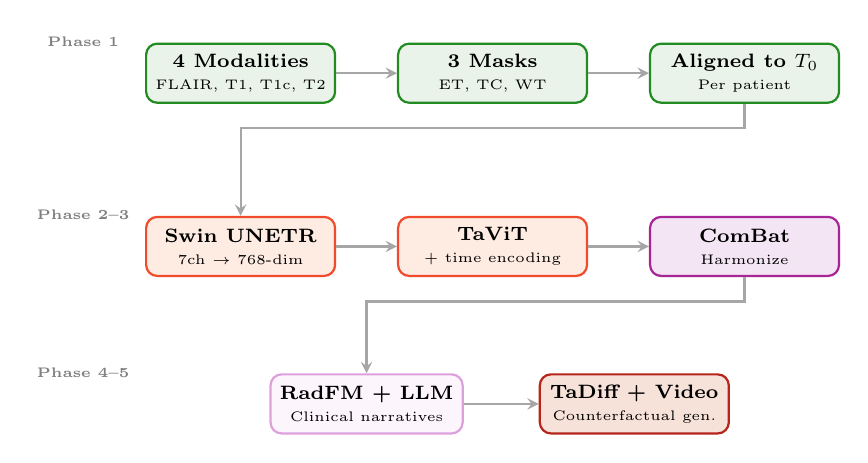
\begin{tikzpicture}[
            box/.style={rectangle, draw=#1, fill=#1!10, thick, minimum height=0.75cm, minimum width=2.4cm, align=center, rounded corners, font=\scriptsize},
            arr/.style={->, thick, >=stealth, color=gray!70},
            lbl/.style={font=\tiny\bfseries, color=gray}
        ]

        % Phase 1 output
        \node[lbl] at (-2,0.4) {Phase 1};
        \node[box=ForestGreen] (mod) at (0,0) {\textbf{4 Modalities}\\{\tiny FLAIR, T1, T1c, T2}};
        \node[box=ForestGreen] (mask) at (3.2,0) {\textbf{3 Masks}\\{\tiny ET, TC, WT}};
        \node[box=ForestGreen] (align) at (6.4,0) {\textbf{Aligned to $T_0$}\\{\tiny Per patient}};

        \draw[arr] (mod) -- (mask);
        \draw[arr] (mask) -- (align);

        % Phase 2-3 input
        \node[lbl] at (-2,-1.8) {Phase 2--3};
        \node[box=RedOrange] (swin) at (0,-2.2) {\textbf{Swin UNETR}\\{\tiny 7ch $\to$ 768-dim}};
        \node[box=RedOrange] (tavit) at (3.2,-2.2) {\textbf{TaViT}\\{\tiny + time encoding}};
        \node[box=Mulberry] (combat) at (6.4,-2.2) {\textbf{ComBat}\\{\tiny Harmonize}};

        \draw[arr] (align) -- ++(0,-0.7) -| (swin);
        \draw[arr] (swin) -- (tavit);
        \draw[arr] (tavit) -- (combat);

        % Phase 4
        \node[lbl] at (-2,-3.8) {Phase 4--5};
        \node[box=Plum] (radfm) at (1.6,-4.2) {\textbf{RadFM + LLM}\\{\tiny Clinical narratives}};
        \node[box=BrickRed] (video) at (5,-4.2) {\textbf{TaDiff + Video}\\{\tiny Counterfactual gen.}};

        \draw[arr] (combat) -- ++(0,-0.7) -| (radfm);
        \draw[arr] (radfm) -- (video);

        \end{tikzpicture}
    \end{center}

    \vspace{0.5em}

    \begin{columns}
        \begin{column}{0.30\textwidth}
            \centering
            \scriptsize
            \textbf{Phase~1 delivers:}\\
            Clean, segmented, aligned MRI
        \end{column}
        \begin{column}{0.35\textwidth}
            \centering
            \scriptsize
            \textbf{Phase~2--3 builds:}\\
            768-dim temporal embeddings
        \end{column}
        \begin{column}{0.30\textwidth}
            \centering
            \scriptsize
            \textbf{Phase~4--5 produces:}\\
            Explanations + counterfactual video
        \end{column}
    \end{columns}
\end{frame}

% ============================================================================
% SLIDE 9: Summary
% ============================================================================
\begin{frame}{Summary}
    \begin{columns}
        \begin{column}{0.48\textwidth}
            \begin{block}{\faIcon{check-circle} Completed}
                \small
                \begin{itemize}
                    \item Full dataset inventory (1,430 patients, 11,877 visits)
                    \item Preprocessing pipeline (registration, resampling, normalization)
                    \item Processed data EDA and quality checks
                    \item CNN baseline (3D CNN + Grad-CAM)
                    \item nnU-Net segmentation notebook (BraTS2021 winner, $\sim$26\,s/case)
                    \item All outputs saved and documented
                \end{itemize}
            \end{block}
        \end{column}

        \begin{column}{0.48\textwidth}
            \begin{alertblock}{\faIcon{arrow-right} Next Steps}
                \small
                \begin{enumerate}
                    \item Run segmentation at scale (996 cases, $\sim$7.2\,h)
                    \item Build registration notebook (itk-elastix)
                    \item (Optional) Validate on Cyprus dataset
                    \item Transition to Phase~2: Swin UNETR embeddings
                \end{enumerate}
            \end{alertblock}

            \vspace{0.3em}

            \begin{exampleblock}{\faIcon{calendar} Timeline}
                \small
                Phase~1 completion: \textbf{$\sim$2 weeks}\\
                Phase~2 start: \textbf{Week~5}\\
                On track for 20-week plan.
            \end{exampleblock}
        \end{column}
    \end{columns}

    \vspace{0.5em}

    \begin{center}
        \large \textbf{Questions?}
    \end{center}
\end{frame}

\end{document}
